\section{Introduction}
\label{sec:introduction}

A moving object can leave its observed position before a robot reaches it.
The same problem arises when a receptacle moves during release or an obstacle
changes the available approach corridor. Dynamic manipulation therefore requires
spatial accuracy at the right time. Faster inference and more responsive
execution reduce observation age \cite{dynamicvla}, while temporal observations
help distinguish motions that look similar in a single image \cite{domino,dynamicwam}.
Together, these demands motivate a practical question:
\emph{what should a robot remember and predict so that its action remains useful
when interaction occurs?}

\begin{figure*}[t]
\centering
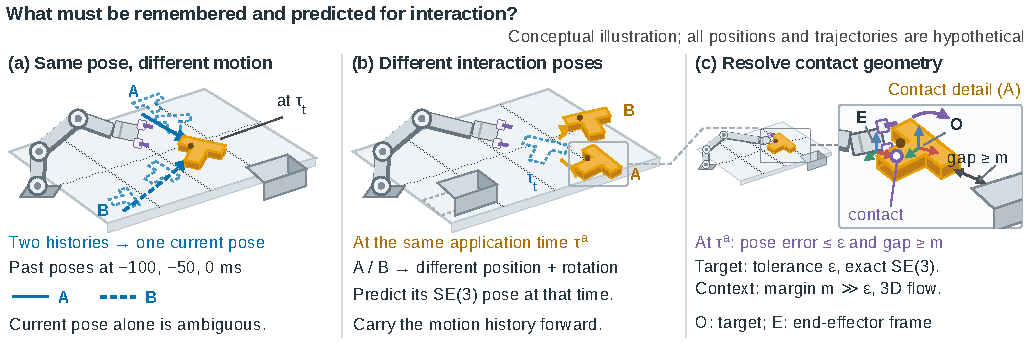
\includegraphics[width=\textwidth]{interaction_timing.pdf}
\caption{What information matters at interaction time?
(a) Two histories meet at the same current target pose.
(b) They lead to different poses at the same future time (solid A, dashed B).
(c) A contact detail for A shows end-effector/target alignment and context clearance.
The same asymmetric target and robot connect the panels. All trajectories
are conceptual illustrations of the research question.}
\label{fig:teaser}
\end{figure*}

The answer depends on the role of information in the task. Target translation
and rotation determine where and how to make contact. A moving occluder or
obstacle matters through its effect on visibility, reachability, or collision.
Static geometry can remain essential even though it has no motion to predict.
This suggests organizing scene evolution by interaction needs: preserve
fine target information when contact requires it, and represent surrounding
changes at sufficient resolution to support the decision. Both a fixed
target/context decomposition and a shared representation with task-dependent
readout can implement this idea. Their relative value is an empirical question.

World--action models provide a framework for learning scene evolution alongside
robot actions \cite{dreamzero,openwam}. However, a future objective changes several
things at once: the supervised variables, the gradients shaping shared features,
and sometimes the computation used before acting. The action may benefit from
auxiliary supervision even when no forecast is generated at deployment
\cite{fastwam}. Conversely, a geometrically accurate forecast may add no useful
information to an already strong state-conditioned policy. Prediction error,
action improvement, and online forecast use must therefore be measured separately.

We organize the \ours Study around three connected questions.
\textbf{Q1} asks how a finite history should encode motion.
\textbf{Q2} asks which future variables, regions, and resolutions support action.
\textbf{Q3} asks how world and action computation should share parameters and
exchange information. Each study matches its own reference; history, future,
and combination studies use distinct recipes. Cross-comparisons revisit
competitive choices before robot-data pretraining.

The completed comparisons give different outcomes across recipes. Structured
GT motion improves the history reference, and a frozen-policy intervention
reveals dependence on its correctness. Visual-history decodability and action
sensitivity do not translate into an overall success-rate advantage.
Among fifteen future-supervision conditions on 1,260 paired scenes, sparse
trajectories give the highest point estimates but no clear overall gain;
dense 2-D displacement decreases success. A twelve-condition combination
screen yields a candidate whose gains over matched controls are concentrated
on phase passage. An adapted DreamVLA system remains stronger under its own
recipe. These results motivate testing how information affects action,
rather than treating added history or future targets as established benefits.

The current evidence supports two contributions:
\begin{itemize}
\item A dynamic-manipulation study protocol that separates task outcomes,
available information, training supervision, and execution conditions.
\item Controlled history and future-supervision studies that distinguish
readable history, action sensitivity, and task benefit, including a frozen-policy
motion-history intervention and fifteen future-supervision conditions.
\end{itemize}
The supplement details the measured configurations and the remaining design,
pretraining, and transfer protocols.
